\documentclass[reprint,
%superscriptaddress,
%groupedaddress,
%unsortedaddress,
%runinaddress,
%frontmatterverbose, 
%preprint,
%preprintnumbers,
nofootinbib,
%nobibnotes,
%bibnotes,
amsmath,amssymb,
aps]{revtex4-1}
\usepackage{physics}
\usepackage{graphicx}
\usepackage{amsmath}
\usepackage{subfigure}
\usepackage{bm}
\usepackage{dcolumn}% Align table columns on decimal point
\usepackage{framed}
\usepackage{empheq}
\usepackage{amsfonts}
\usepackage{esint}
\usepackage[makeroom]{cancel}
\usepackage{dsfont}
\usepackage{centernot}
\usepackage{mathtools}
\usepackage{bigints}
\usepackage{empheq}
\usepackage{tensor}
\usepackage{xcolor}
\definecolor{colby}{rgb}{0.0, 0.0, 0.5}
\definecolor{MIT}{RGB}{163, 31, 52}
\usepackage[pdftex]{hyperref}
%\hypersetup{colorlinks,linkcolor={MIT},citecolor={MIT},urlcolor={MIT}}  
\hypersetup{colorlinks,linkcolor=blue,citecolor=blue,urlcolor=blue}  
%\usepackage[left=1in,right=1in,top=1in,bottom=1in]{geometry}
%\setcounter{MaxMatrixCols}{20}
% \usepackage{newpxtext,newpxmath}
%\newcommand*\widefbox[1]{\fbox{\hspace{2em}#1\hspace{2em}}}

\newcommand{\p}{\partial}
\newcommand{\R}{\mathbb{R}}
\newcommand{\C}{\mathbb{C}}
\newcommand{\lag}{\mathcal{L}}
\newcommand{\nn}{\nonumber}
\newcommand{\ham}{\mathcal{H}}
\newcommand{\M}{\mathcal{M}}
\newcommand{\I}{\mathcal{I}}
\newcommand{\K}{\mathcal{K}}
\newcommand{\F}{\mathcal{F}}
\newcommand{\w}{\omega}
\newcommand{\lam}{\lambda}
\newcommand{\al}{\alpha}
\newcommand{\be}{\beta}
\newcommand{\x}{\xi}
\newcommand{\G}{\mathcal{G}}
\newcommand{\f}[2]{\frac{#1}{#2}}
\newcommand{\ift}{\infty}
\newcommand{\lp}{\left(}
\newcommand{\rp}{\right)}
\newcommand{\lb}{\left[}
\newcommand{\rb}{\right]}
\newcommand{\lc}{\left\{}
\newcommand{\rc}{\right\}}
\newcommand{\V}{\mathbf{V}}
\newcommand{\U}{\mathcal{U}}
\newcommand{\Id}{\mathcal{I}}
\newcommand{\D}{\mathcal{D}}
\newcommand{\Z}{\mathcal{Z}}

\definecolor{gris245}{RGB}{245,245,245}
\definecolor{olive}{RGB}{50,140,50}
\definecolor{brun}{RGB}{175,100,80}

\newcommand{\diag}{\text{diag}}
\newcommand{\psirot}{\ket{\psi_\text{rot}(t)} }
\newcommand{\RWA}{\ham_\text{rot}^\text{RWA}}

% 3j symbol
\newcommand{\tj}[6]{ \begin{pmatrix}
		#1 & #2 & #3 \\
		#4 & #5 & #6 
\end{pmatrix}}



\begin{document}
	
	

\title{Linear response theory and applications in ultracold atom experiments}
\author{Huan Q. Bui}
\email{huanbui@mit.edu}
\affiliation{
	MIT-Harvard Center for Ultracold Atoms, Research Laboratory of Electronics, and Department of Physics, Massachusetts Institute of Technology, Cambridge, Massachusetts 02139, USA}
\date{\today}


\begin{abstract}
	In this paper, we study linear response theory and its applications in AMO physics. We begin by introducing and reviewing the basic aspects of linear response theory in the language of classical and and statistical mechanics and generalize to quantum mechanics. We then show the power of this formalism by reviewing its role in deriving important results such as the Kubo formula and the fluctuation-dissipation theorem. Finally, we apply these results and the linear response approach to extract physics of two exemplary many-body quantum systems, namely the weakly-interacting Bose-Einstein condensate (BEC) and the Fermi gas with interactions.
\end{abstract}

\maketitle


\section{Introduction}



It is often possible to solve for the dynamics of single-body $N$-level systems exactly, either analytically or numerically. For example, Rabi oscillations perfectly describe the dynamics of a two-level system. However, many-body systems such as non-ideal BECs or the unitary Fermi gas often exhibit complicated interactions, making exact descriptions of these systems unattainable in most cases. As a result, solutions typically come from linear response theory. 

The object of study in linear response theory is the response function. In the simplest case, the response function is a proportionality constant $\chi$ relating the response of a system $x(t)$ due to a perturbation $h(t)$ at that instant $t$. For linear, time-invariant systems with memory, the response $x(t)$ is the convolution of the response function with the perturbation:
\begin{align}\label{eq:linear_response}
x(t) = \int_{-\infty}^{\infty} \chi(t-t') h(t') \,dt'.
\end{align}
In general, $\chi$ solves the equation $ L \chi(t-t') = \delta(t-t')$ where $L$ is the linear differential operator associated with the system under consideration. It is identically the Green's function associated with $L$ and characterizes the system's response to an external impulse. As Sections \ref{sec:classical} and \ref{sec:quantum} will show, linear response theory provides a means for extracting rich physics for a range of physical systems from a damped harmonic oscillator to a canonical ensemble in statistical physics to quantum gases with many-body interactions. 


\section{Classical Linear Response}\label{sec:classical}

%
\subsection{Causality}
The response function tells us how a system responds \textit{as a consequence} of some perturbation, which means it respects causality, i.e., $\chi(t) = 0$ for $t < t_0 = 0$ when the perturbation is turned on. Consider $\chi(t)$ in Fourier basis:
\begin{align*}
\chi(t) = \int_{-\infty}^\infty  e^{-i\omega t } \tilde{\chi}(\omega) \,d\omega.
\end{align*}
For $t<0$, we integrate by closing the contour in the upper half-plane. Since the answer is zero, $\chi(\omega)$ must be analytic in the upper half-plane. In other words, 
\begin{align*}
\text{Causality} \implies \chi(\omega) \text{ analytic for } \Im(\chi) > 0.
\end{align*}
Let $\chi'(\omega) = \Re \chi(\omega)$ and $\chi''(\omega) = \Im \chi(\omega)$. $\chi'(\omega)$ is called the \textit{reactive part} of the response, and $\chi''(\omega)$ the \textit{dissipative part}. SInce $\chi(t)$ is invariance under time translations, one can show that $\chi'(\omega)$ and $\chi''(\omega)$ are even and odd functions, respectively.

If $\chi(\omega)$ decays faster than $1/\abs{\omega}$ as $\omega \to \infty$ in addition to being analytic in the upper half-plane, then $\chi'(\omega)$ and $\chi''(\omega)$ are related via the Kramer-Kronig relations. In particular, one can reconstruct the full complex response function knowing only its imaginary part:
\begin{align*}
\chi(\omega) = \int_{-\infty}^\infty \f{d\omega'}{\pi} \f{\Im \chi'(\omega')}{\omega' - \omega - i\epsilon}.
\end{align*}

As an example, let us consider the damped driven harmonic oscillator. We can fully characterize its resonance behavior and energy dissipation based solely on the (complex) response function. Fourier-transforming the equation of motion and using  \eqref{eq:linear_response} give the response function in frequency domain:
\begin{align*}
\ddot{x} + \gamma \dot{x} + \omega_0^2 x = h(t) \implies 
\tilde{\chi}(\omega) = ( \omega_0^2 - \omega^2 - i \gamma \omega)^{-1}.
\end{align*}
The static response function is $\tilde{\chi}(\omega = 0) = 1/\omega_0^2$, giving $x = h/\omega_0^2$ as expected. For a drive with frequency $\omega$, the response function has poles $\omega_\star$ given by 
\begin{align*}
\omega_* = -i\gamma/2 \pm \sqrt{\omega_0^2  - \gamma^2/4}.
\end{align*}
When the oscillator is underdamped $(\gamma/2 < \omega_0)$, the poles have both real and imaginary parts and are in the lower half-plane. When the oscillator is overdamped $(\gamma/2 > \omega_0)$, the poles are on the negative imaginary axis. In both cases, $\tilde{\chi}(\omega)$ is analytic in the upper half-plane, consistent with causality. 

Suppose the drive is $h(t) = h_0 \Re(e^{-i\omega t})$ and that the system is in steady state. The average power dissipated by the system is the average power absorbed: 
\begin{align*}
\langle P \rangle = 2h_0^2 \omega \Im\widetilde{\chi}(\omega) = 2h_0^2  \gamma \omega^2 [(\omega_0^2 - \omega^2)^2 + \gamma^2 \omega^2]^{-1},
\end{align*}
which has a Lorentzian line shape with FWHM $\gamma$ near resonance. Note that the first equality holds in general and depends only on $\Im \widetilde{\chi}(\omega)$.
%
\subsection{Response function and correlation function}
The following discussion follows  Chapter 8 of \cite{chandler1988introduction} and Chapter 7 of \cite{chaikin1995principles}. Let us generalize a bit and apply the idea of linear response theory to a canonical ensemble that is perturbed out of equilibrium. Let $\mathcal{H}$ be the unperturbed Hamiltonian and consider some dynamical variable $A$, which is a function defined over the phase space for the system. The equilibrium average for $A$ is:
\begin{align*}
\langle A \rangle =  \mathcal{Z}^{-1}(\mathcal{H}) \int e^{-\be \mathcal{H}} A\, d\Omega,
\end{align*}
where $\mathcal{Z}(\mathcal{H}) = \int e^{-\be \mathcal{H}} \, d\Omega$, and $\int \cdot \,d\Omega$ is an integral over phase space. Next, suppose the system is initially perturbed by $\Delta \mathcal{H} = -f A$ where $f$ is some external field. We are interested in what happens to the non-equilibrium average $\overline{A}$ as time progresses. This quantity is given by 
\begin{align*}
\overline{A}(t) = \mathcal{Z}^{-1}(\mathcal{H} + \Delta \mathcal{H})  \int e^{-\be(\mathcal{H} + \Delta \mathcal{H})} A(t) \, d\Omega. 
\end{align*}
For $t>0$, $\Delta \mathcal{H}$ vanishes, so it is $\mathcal{H}$ that governs the time evolution of $A(t)$. Assuming that the perturbations are small, i.e. $A(t)$ does not deviate much from $\langle A \rangle$, we can find $\overline{A}(t)$ in terms of $A$ with corrections due to $\Delta \mathcal{H}$:
\begin{align*}
\overline{A}(t) 
%&= \f{\int e^{-\be \mathcal{H} (1- \be \Delta \mathcal{H} + \dots )A(t) \,d\Omega}}{\int e^{-\be \mathcal{H} (1 - \be \Delta \mathcal{H}) + \dots } \, d\Omega } \\ 
&\approx \mathcal{Z}^{-1}(\mathcal{H})  \int d\Omega \, e^{-\be \mathcal{H}} A(t)   \lb 1 - \be \Delta \mathcal{H}  + \langle  \be \Delta \mathcal{H}  \rangle  \rb \\ 
&= \langle A \rangle - \be \lb \langle \Delta \mathcal{H} A(t) \rangle - \langle A \rangle \langle \Delta \mathcal{H} \rangle  \rb.
\end{align*}
Insert the expression for $\Delta \mathcal{H}$ into the result above to get
\begin{align}
\label{eq:fluctuation}
\Delta \overline{A}(t) = \be f \langle \delta A(t) \delta A(0) \rangle + {O}(f^2),
\end{align}
where $\Delta \overline{A}(t) = \overline{A}(t) - \langle A \rangle$ is the (averaged, thus macroscopic) spontaneous fluctuation, and $\delta A(t) = A(t) - \langle A \rangle$ is the (microscopic) instantaneous fluctuation at time $t$. This is a remarkable result that we just showed: the spontaneous fluctuations is related to the time correlation function of instantaneous fluctuations. Since generally, $\langle \delta A \rangle = 0$ but $\langle A^2 \rangle \neq 0$, we see that $\Delta \overline{A}(t)$ decays in time. This is the essence of Onsanger's remarkable \textit{regression hypothesis} which was later realized to be a consequence of the fluctuation-dissipation theorem (FDT), which we will briefly discuss in Section \ref{sec:quantum}.

We now write $\Delta \overline{A}(t)$ in terms of $\chi(t-t')$:
\begin{align}
\label{eq:fluctuation_response_function}
\Delta \overline{A}(t) = \int_{-\infty}^\infty dt' \chi(t-t') f(t'). 
\end{align}
For convenience, consider $f(t) = f \Theta(-t)$ which tells us that the perturbation is turned off at $t=0$, then we quickly find
\begin{align*}
\Delta \overline{A}(t) = f \int_{t}^\infty \chi(t') \,dt'.
\end{align*}
By comparing this with \eqref{eq:fluctuation}, we find that
\begin{align*}
\chi(t) = -\be \f{d}{dt} \langle \delta A(0) \delta A(t) \rangle \Theta(t).
\end{align*}
We see that the response function for a non-equilibrium system is related to the correlations between spontaneous fluctuations at different times as they occur in the equilibrium system.


%
\section{Quantum Linear Response}\label{sec:quantum}

The following discussion follows Chapter 8 of \cite{chandler1988introduction}, Chapter 7 of \cite{chaikin1995principles}, and notes by Professor David Tong \cite{tong2012kinetic} and Professor Habib Rostami \cite{rostamilecture}.

\subsection{Overview}
The treatment of linear response theory in quantum mechanics is similar to the classical case, with the exception that functions become operators, which do not commute in general. Let the dynamics of a generic quantum system be governed by a bare Hamiltonian $\mathcal{H}$ and let a small perturbation be $\mathcal{H}'(t)$ which turns on for $t\geq t_0$. In the interaction picture, the states evolve as $\ket{\psi(t)}_I = U(t,t_0) \ket{\psi(t_0)}_I$, where
\begin{align*}
U(t,t_0) 
&= \mathcal{T} \exp\lp -i \int_{t_0}^t  \mathcal{H}'(t')\,dt'\rp.
\end{align*}
Suppose we are interested in an observable $\mathcal{O}$. By expanding $U(t,t_0)$ to second order in $\mathcal{H}'$, we can approximate the expectation value of $\mathcal{O}$ at time $t$:
\begin{align}
\label{eq:time-evolution}
\langle \mathcal{O}(t) \rangle_{\phi} = \langle \mathcal{O}(t) \rangle_{0} + i \int_{-\infty}^t dt' \langle [\mathcal{H'}(t'), \mathcal{O} (t)] \rangle_{0} + \dots
\end{align}
Here, the $0$ subscript denotes evaluation using $\ket{\psi(t_0)}$.  This result is known as Kubo's formula. 

Suppose that the perturbation Hamiltonian has the form $\mathcal{H}'(t) = \sum_j \phi_j (t) \mathcal{O}_j(t)$, with an implicit sum over $j$ and let $\delta \langle \mathcal{O}_i \rangle = \langle \mathcal{O}_i \rangle_\phi - \langle  \mathcal{O}_i \rangle_{\phi = 0}$ denote the deviation of the observable from its equilibrium value, we have
\begin{align*}
\delta \langle \mathcal{O}_i \rangle 
&=  i \int_{-\infty}^t dt' \langle  [ \mathcal{O}_j(t'), \mathcal{O}_i(t)   ] \rangle \phi_j(t') \\
&= i \int_{-\infty}^\infty dt' \Theta(t-t') \langle  [ \mathcal{O}_j(t'), \mathcal{O}_i(t)   ] \rangle \phi_j(t').
\end{align*} 
Comparing this to \eqref{eq:linear_response} and \eqref{eq:fluctuation_response_function}, we can identify that the response function for the system is a two-point correlation function, similar to what we did in Section \ref{sec:classical}:
\begin{align}\label{eq:corr_func}
\chi_{ij}(t-t') = -i \Theta(t-t') \langle  [ \mathcal{O}_j(t'), \mathcal{O}_i(t)   ] \rangle,
\end{align}
which is a more specific version of the Kubo's formula. By further assuming that the system is a canonical ensemble and going to Fourier space, the response function takes a more familiar form:
\begin{align*}
\widetilde{\chi}_{ij}(\omega) = \sum_{m,n} e^{-\be E_m} \lb 
\f{(\mathcal{O}_j)_{mn}(\mathcal{O}_i)_{mn}}{\omega - \omega_{nm} + i\epsilon} 
- 
\f{(\mathcal{O}_i)_{mn}(\mathcal{O}_j)_{mn}}{\omega + \omega_{nm} + i\epsilon} 
\rb.
\end{align*}
Formal properties of $\widetilde{\chi}$ can be studied from this representation. While they are beyond the scope of this review, the reader may refer to \cite{pitaevskii2016bose} for more details.  


\subsection{Measurements, correlation functions, and FDT}
While the Kubo formula seems rather abstract, we may recall that correlation functions are experimental observables. Consider the transition probability $S(\omega)$ which follows Fermi's golden rule:
\begin{align*}
\widetilde{S}(\omega) = \sum_{nm} P_m \abs{ \bra{\psi_n} \mathcal{O} \ket{\psi_m}  }^2  \delta(\omega - \omega_{nm}) 
\end{align*}
where $P_m$ is some equilibrium distribution to account for finite temperature. By Fourier transforming, we can relate $\widetilde{S}(\omega)$ back to a correlation function like in \eqref{eq:corr_func}:
\begin{align*}
S(\tau) = (2\pi)^{-1}\langle \mathcal{O}(\tau) \mathcal{O}^\dagger(0) \rangle. 
\end{align*}
In general, one can \textit{define} $\widetilde{S}(\omega)$, called the \textit{dynamic structure factor} as:
\begin{align*}
\widetilde{S}(\omega) 
&= \f{1}{2\pi}\int_{-\infty}^\infty \langle \mathcal{O}(t) \mathcal{O}^\dagger (0) \rangle e^{i \omega t }\,dt\\
&= \abs{\mathcal{O}_0}^2 \delta(\omega) + \f{1}{2\pi} \int_{-\infty}^\infty \langle \delta \mathcal{O}(t) \delta \mathcal{O}^\dagger (0) \rangle e^{i\omega t }\,dt,
\end{align*}
where $ \mathcal{O} = \mathcal{O}_0 + \delta \mathcal{O}$, and $\langle \delta \mathcal{O} \rangle = 0$. For $ \omega \neq 0$, we see that $\widetilde{S}(\omega)$ captures the dynamics of the fluctuations of $\mathcal{O}$. Assuming $P_m \sim e^{-\be \omega_m}$, one can prove the fluctuation-dissipation theorem:
\begin{align*}
\Im \widetilde{\chi}(\omega) = \pi[\widetilde{S}(\omega) - \widetilde{S}(-\omega)] = \pi (1 - e^{-\be \omega}) S(\omega),
\end{align*}
which relates fluctuations, captured by $\widetilde{S}(\omega)$, to dissipation in the system, captured by the imaginary part of the response function, just like in the damped harmonic oscillator example. We also notice that while at zero temperature, $\Im \widetilde{\chi}(\omega)$ and $S(\omega)$ for all $\omega >0$, the two functions differ significantly for $T \neq 0$ with $\widetilde{S}(\omega)$ having stronger $T$-dependence. As a result, the dynamic structure factor is a more fundamental quantity for many-body theory. For a highly pedagogical treatment of the FDT and its history, the reader may refer to \cite{marconi2008fluctuation}.




\section{Applications}
In this section, we review some applications of linear response theory in ultracold atom experiments. In Section \ref{sec:Bose}, we calculate the structure factors for a Bose gas in both the ideal and weakly-interacting case. In Section \ref{sec:spec}, we survey how the linear response formalism is used to derive spectra of quantum gases from first principles.

\subsection{Density response of a Bose gas}
\label{sec:Bose}
This section closely follows Chapter 7 of \cite{pitaevskii2016bose}. Consider the density operator for a Bose gas $n(\mathbf{r}) = \sum_i \delta(\mathbf{r} - \mathbf{r}_i)$. The $\mathbf{q}$-component of this operator in Fourier space is $\widetilde{n}_\mathbf{q} = \sum_i e^{-i \mathbf{q}\cdot \mathbf{r}}$. From the formalism in the Section \ref{sec:quantum}, the Fourier-space density response function is
\begin{align*}
\widetilde{\chi}(\mathbf{q},\omega) = \sum_{m,n} e^{-\be E_m} 
\lb 
\f{\abs{\delta \widetilde{n}_{\mathbf{q},mn}}^2}{\omega - \omega_{mn} + i\eta} 
- 
\f{\abs{\delta \widetilde{n}_{\mathbf{q},mn}^\dagger}^2}{\omega + \omega_{mn} + i\eta} 
\rb
\end{align*}
Here we have dropped the normalization pre-factor $-1/(\hbar \mathcal{Z})$ for convenience and $\delta \widetilde{n}_{\mathbf{q},mn} = \bra{m} \delta \widetilde{n}_{\mathbf{q}} \ket{n}$, where $\delta \widetilde{n}_\mathbf{q} = \widetilde{n}_\mathbf{q} - \langle \widetilde{n}_\mathbf{q} \rangle_\text{eq}$ is the deviation from equilibrium. Similarly, the dynamic structure factor is 
\begin{align*}
\widetilde{S}(\mathbf{q},\omega) = \sum_{m,n} e^{-\be E_m} \abs{\delta \widetilde{n}_{\mathbf{q},mn}}^2 \delta(\hbar \omega - \hbar \omega_{mn}).
\end{align*}
In words, the dynamic structure factor $\widetilde{S}(\mathbf{q},\omega)$ is the Fourier transform of the density-density correlation function. It describes all excitations available in the system at frequency $\omega$ and momentum $\mathbf{q}$. 

\subsubsection{Ideal Bose gas}

The density response function of an ideal Bose gas can be calculated analytically. The key is to calculate the matrix element $\delta \widetilde{n}_{\mathbf{q},mn}$. This is done by rewriting $\widetilde{n}_\mathbf{q}$ in second-quantization: $\widetilde{n}_\mathbf{q} = \sum_\mathbf{p} a^\dagger_{\mathbf{p} - \hbar \mathbf{q}} a_\mathbf{p} $. Since the eigenstates of the Hamiltonian describing the ideal Bose gas are fixed by occupation numbers $f_\mathbf{q}$ of each single-particle state, the matrix element $\bra{m} a^\dagger_{\mathbf{p} - \hbar \mathbf{q}} a_\mathbf{p} \ket{n}$ vanishes unless the energy difference $E_n - E_m$ is equal to the difference in single-particle energies $\epsilon(\mathbf{p} + \hbar \mathbf{q}) - \epsilon(\mathbf{p})$. One can then show that the dynamic structure factor and the imaginary part of the density response function are:
\begin{align*}
\widetilde{S}(\mathbf{q},\omega) &= \sum_\mathbf{p} f_\mathbf{p}(1 + f_{\mathbf{p} + \hbar \mathbf{q}}) \delta 
\lp
\hbar \omega - \f{\hbar^2 q^2}{ 2m} - \f{\hbar }{m} \mathbf{q}\cdot \mathbf{p}
\rp \\
\widetilde{\chi}''(\mathbf{q},\omega) 
&= 
\pi \sum_\mathbf{p} (f_\mathbf{p} - f_{\mathbf{p} + \hbar \mathbf{q}}) \delta 
\lp  
\hbar \omega - \f{\hbar^2 q^2}{ 2m} - \f{\hbar }{m} \mathbf{q}\cdot \mathbf{p}
\rp.
\end{align*}
Here, $f_\mathbf{p} = \langle a^\dagger_\mathbf{p} a_\mathbf{p}\rangle$ is the Bose-Einstein distribution. In the presence of the BEC, one separates the contribution from the BEC and integrate the rest over $\mathbf{p}$ to get
\begin{align*}
\widetilde{\chi}''(\mathbf{q},\omega) &= \pi  N_0(T) \delta \lp \hbar \omega - \f{\hbar^2 q^2}{2m} \rp  \\
 + \, \pi &\int d\mathbf{p} f'_\mathbf{p} \delta \lp \hbar \omega - \f{\hbar^2 q^2}{2m} - \f{\hbar}{m} \mathbf{p}\cdot \mathbf{p} \rp - [\omega \to -\omega], 
\end{align*}
where $f'_\mathbf{p} = f_\mathbf{p} - N_0 \delta(\mathbf{p})$ is the momentum distribution for particles not in the condensate. $\widetilde{\chi}(\mathbf{q},\omega)$ has two $\delta$-function peaks at $\omega = \pm \hbar q^2/2m$ and a continuum of excitations from the thermal part of the gas. For $T \ll T_c$, we have $N_0(T) \approx N$, implying $\widetilde{\chi}''(\mathbf{q},\omega)$ is reduced to just the $\delta$-functions parts and  
\begin{align*}
\widetilde{S}(\mathbf{q},\omega) = \f{N}{1 - e^{-\hbar \omega / k_BT}} \lb \delta\lp \omega - \f{\hbar q^2}{2m} \rp - \delta \lp  \omega + \f{\hbar q^2}{2m} \rp \rb.
\end{align*}
which has strong temperature dependence, unlike $\widetilde{\chi}''(\mathbf{q},\omega)$.  Integrating out the $\omega$-dependence of $\widetilde{S}(\mathbf{q},\omega)$ gives the \textit{static structure factor}
\begin{align*}
\widetilde{S}(\mathbf{q}) = \coth \f{\hbar^2 q^2}{4mk_BT},
\end{align*}
which approaches $1$ for large $q$ and diverges for small $q$, reflecting the infinite compressibility for the ideal Bose gas at the BEC transition \cite{kardar2007statistical}. As we will see in the next section, $\widetilde{S}(\mathbf{q})$ approaches a finite value in the presence of interactions. 

\begin{figure}[!htb]
\label{fig:ideal}
\centering
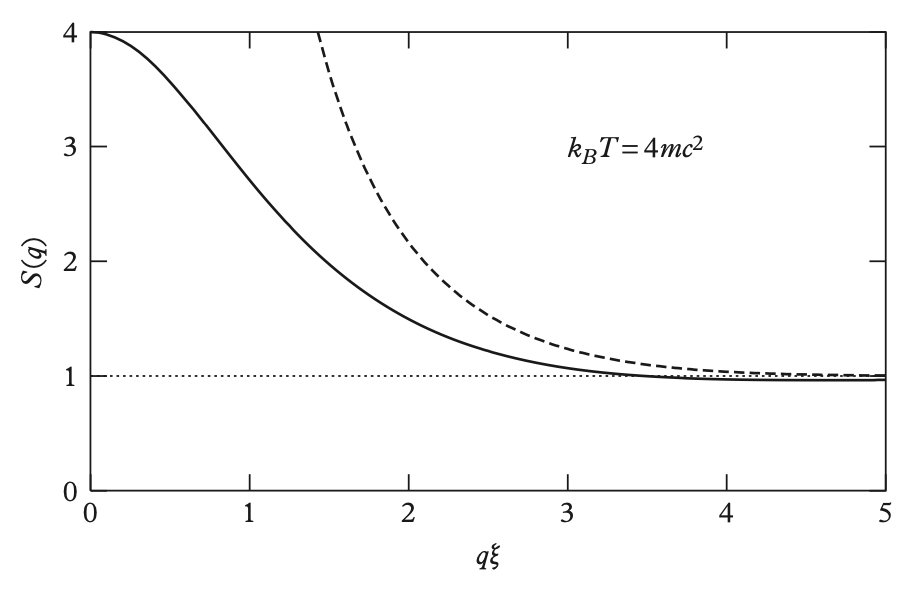
\includegraphics[width=0.3\textwidth]{figures/ideal.png}
\caption{$\widetilde{S}(\mathbf{q})$ for the Bose gas as a function of non-dimensionalized $q$ at $k_BT / mc^2 = 4$. The black (dashed) line corresponds to the case with(out) interactions \cite{pitaevskii2016bose}.}
\end{figure}


\subsubsection{Weakly-interacting Bose gas}
Bogoliubov theory provides a good treatment for the Bose gas with weak interactions $(na^3\ll1)$ where the gas is mostly the condensate $(T\ll T_c)$ and . The derivation of the dynamic and static structure factors follows the same path as in the previous section, with the exception that density operator is redefined in terms of the creation and annihilation operators are those for quasiparticles. While Bogoliubov theory is beyond the scope of this paper, we are interested in the result for the imaginary part of the density response function:
\begin{align*}
\widetilde{\chi}''(\mathbf{q},\omega) = \pi \f{\hbar^2 q^2 N}{2m \epsilon(\mathbf{\hbar q})} 
[\delta(\hbar \omega - \epsilon(\mathbf{\hbar q})) - \delta(\hbar \omega + \epsilon(\mathbf{\hbar q}))],
\end{align*}
where $\epsilon(\mathbf{q})$ is the Bogoliubov energy of elementary excitations $\epsilon(p) = \sqrt{gNp^2/mV + (p^2/2m)^2}$ with $g$ being the coupling strength. The dynamic structure factor thus takes the form
\begin{align*}
\widetilde{S}(\mathbf{q},\omega) 
&= \f{\hbar^2 q^2 N}{2m\epsilon(\mathbf{\hbar q})} \f{1}{1-e^{-\hbar \omega/k_BT}} \\
&\quad\times[\delta(\hbar \omega - \epsilon(\mathbf{\hbar q})) - \delta(\hbar \omega + \epsilon(\mathbf{\hbar q}))],
\end{align*}
The static structure factor is thus 
\begin{align*}
\widetilde{S}(\mathbf{q}) = \f{\hbar^2 q^2}{2m\epsilon(\mathbf{\hbar q})} \coth \f{\epsilon(\hbar\mathbf{q})}{2k_BT}
\end{align*}
which generalizes the result for the ideal Bose gas and reduces to $\hbar^2 q^2/2m\epsilon(\hbar \mathbf{q})$ for $T = 0$. For large $q$, the static structure factor saturates to unity as $\widetilde{S}(\mathbf{q}) \sim 1 - 2m^2c^2 / \hbar^2 q^2$ where $c = \sqrt{gn/m}$ is the speed of sound. For finite $T$ but low $q$, $\widetilde{S}(\mathbf{q})$ approaches $k_BT / mc^2$ rather than diverging like in the case of the ideal Bose gas. This is due to interactions: thermal excitations of phonons become important at small $q$, keeping $\widetilde{S}(\mathbf{q})$ finite in accordance with the fluctuation-dissipation theorem. For a more detailed derivation of these results (beyond the level of detailed provided by \cite{pitaevskii2016bose}), see \cite{yukalov2007structure}. 

An interesting feature is that for $T \ll T_c$, $\widetilde{\chi}''(\mathbf{q},\omega)$ is essentially its $T=0$ value. However, $\widetilde{S}(\mathbf{q})$ still has a strong dependence on temperature, as shown in Figures \ref{fig:ideal} and \ref{fig:interacting}. 

\begin{figure}[!htb]
\label{fig:interacting}
\centering
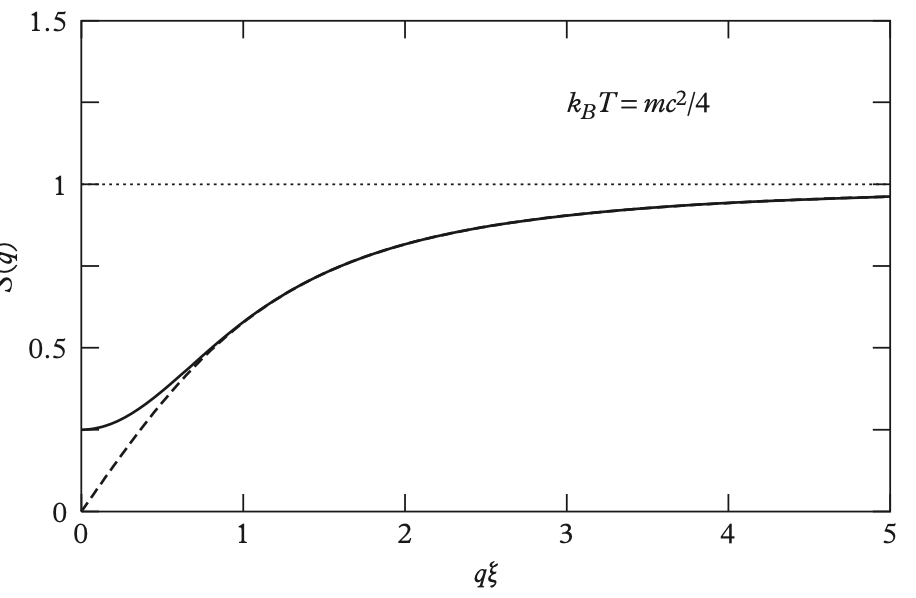
\includegraphics[width=0.3\textwidth]{figures/interacting.png}
\caption{$\widetilde{S}(\mathbf{q})$ for a weakly-interacting BEC as a function of non-dimensionalized $q$. The dashed and black lines correspond to $k_BT/mc^2=0$ and $k_BT/mc^2 = 1/4$, respectively \cite{pitaevskii2016bose}.}
\end{figure}
\subsubsection{Experimental results}

In \cite{hung2011extracting}, the static structure factor for different values of the coupling constant was measured for the two-dimensional Bose gas using \textit{in situ} imaging. The results show explicitly the different behavior of $\widetilde{S}(\mathbf{q})$ at small $q$ for different values of $k_BT / mc^2$, similar to what we see in Figures \ref{fig:ideal} and \ref{fig:interacting}, Figure \ref{fig:hung2011} shows the \textit{in situ} density fluctuations and the static structure factors for the weakly-interacting 2D Bose gas extracted from these images. 
\begin{figure}[!htb]
\label{fig:hung2011}
\centering
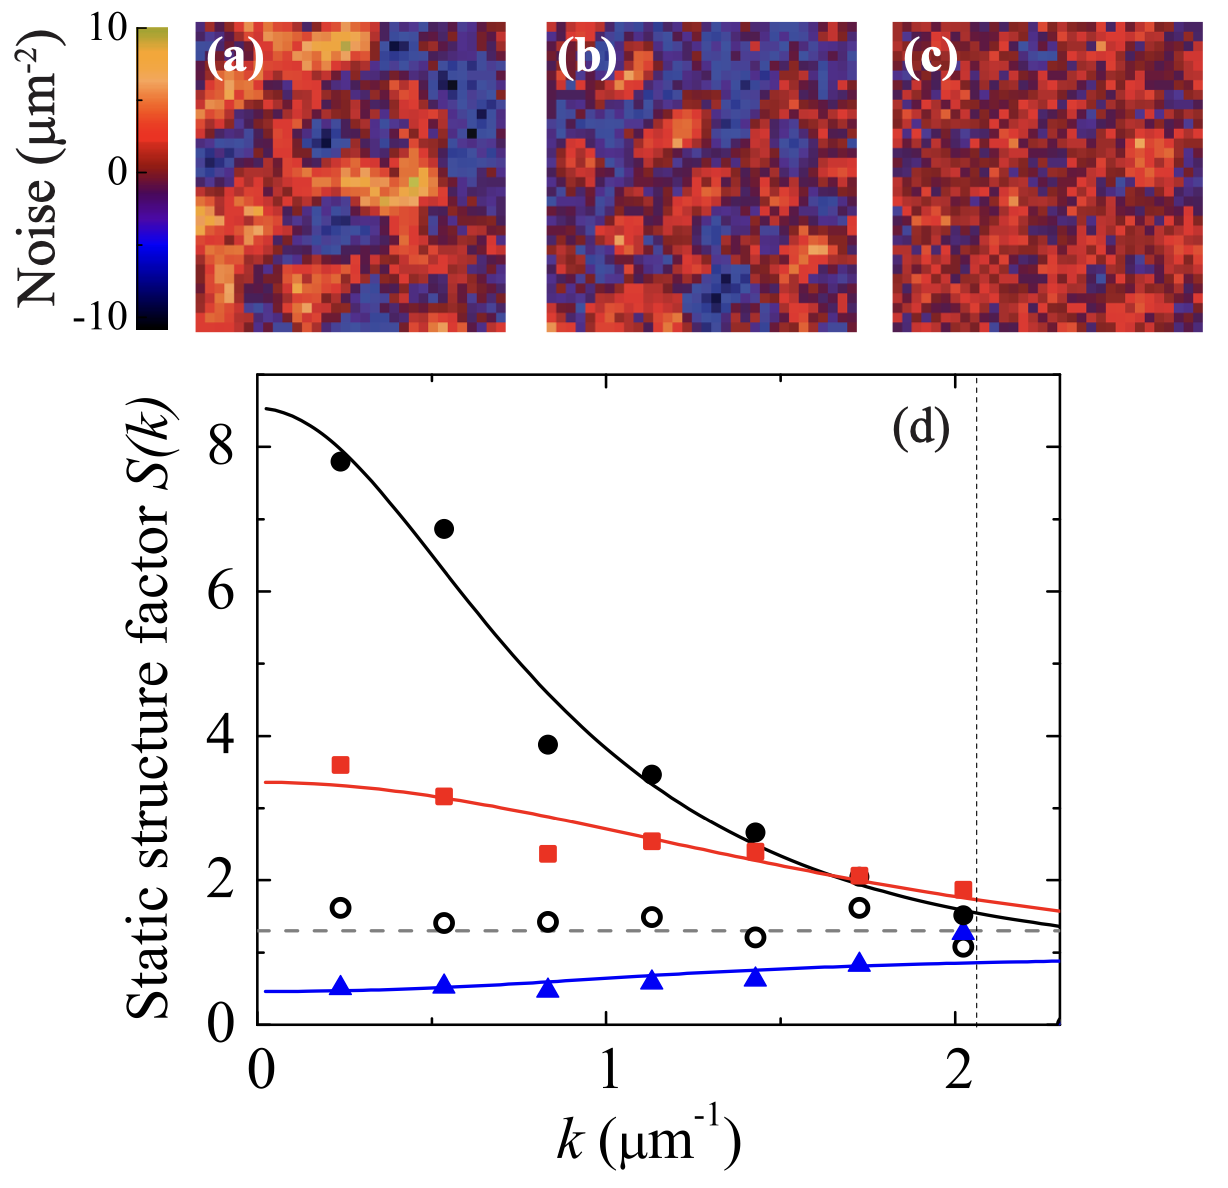
\includegraphics[width=0.3\textwidth]{figures/hung2011.png}
\caption{Density fluctuations and the static structure factors. (a), (b), (c): image noise for 2D Bose gases with coupling constant $g = 0.05, g = 0.26,$ and $g_\text{eff} = 1.0$. (d) shows $\widetilde{S}(\mathbf{q})$ extracted from the noise power spectra from (a) (black circles), (b) (red squares), and (c) (blue triangles). Open circles denote $\widetilde{S}(\mathbf{q})$ of an ideal thermal gas at $n\lambda_{dB}^2$ = 0.5. }
\end{figure}

The (momentum-resolved) dynamic structure factor $\widetilde{S}(\mathbf{q},\omega)$ for a BEC has been measured directly via Bragg spectroscopy \cite{stenger1999bragg}. As we will see in \ref{sec:spec}, spectroscopy of quantum gases, including Bragg spectroscopy, can also be understood from the linear response formalism. 




\subsection{Spectroscopy of quantum gases}\label{sec:spec}

The linear response formalism allows one to derive spectra of many-body quantum systems from first principles. In almost all cases, we can reveal physical properties of quantum systems by showing how they couple to external fields such as RF or optical light. For example, the RF spectrum of a BCS superfluid of $^6$Li displays a threshold behavior due to the superfluid gap and a long tail due to the BCS dispersion \cite{schirotzek2008determination}, \cite{torma2014quantum}. In this section, we provide a high-level description for how spectra is calculated for a quantum many-body system from first principles and linear response. We then review some exemplary results from these calculations and compare them to experimental results. A fully rigorous and pedagogical treatment of this topic is far beyond the scope of this paper, but can be found in Chapter 10 of \cite{torma2014quantum}. 
 
\subsubsection{RF spectra from linear response}\label{sec:method}

In typical RF spectroscopy, the RF field drives a transition between two internal states of the atoms. Atoms in the initial state could be interacting, giving rise to shifts, while atoms in the final state are ideally non-interacting.  The general scheme for obtaining spectra of a many-body system interacting with a field from the linear response formalism is as follows. Consider a system with two interacting fermionic species $a$ and $(b)$. We first write down the full Hamiltonian $\mathcal{H}$ containing the "bare" energies of the species (kinetic energy, internal state energy, and external trapping potential), the interparticle interaction potential, field $\Omega_{ab}(\mathbf{r},t)$ that couples the two species, and (optionally) the chemical potential. When calculating the response of the system to $\Omega_{ab}(\mathbf{r},t)$, we isolate the part of $\mathcal{H}$ that contains $\Omega_{ab}$ and calculate the time evolution of, say, the rate of change of the counts of species $b$, using \eqref{eq:time-evolution}, assuming the long time and weak perturbation limit. Under the rotating-wave approximation, this quantity has the form
\begin{align*}
\langle \dot N_b(t) \rangle &\sim \int_{t_0}^t dt' \int d^3 r  d^3 r' \Omega(\mathbf{r}) \Omega^*(\mathbf{r}') e^{-i \widetilde{\delta}(t-t')}  \times \\
& \langle [\hat{\psi}_b^\dagger (\mathbf{r},t) \hat{\psi}_a (\mathbf{r},t), \hat{\psi}_a^\dagger (\mathbf{r}',t') \hat{\psi}_b (\mathbf{r}',t') ] \rangle+ \text{h.c.}
\end{align*} 
where the $\hat{\psi}$ are field operators and $\widetilde{\delta} = \delta + (\mu_b - \mu_a)/\hbar$ is the generalized detuning with $\mu_i$ being the chemical potential. In usual RF spectroscopy where the initial and final states of the system do not interact or interact weakly, the correlation term can be factorized or approximated. To evaluate them, we write the field operators in terms of known basis functions and creation/annihilation operators $\hat{\psi}_a^\dagger(\mathbf{r},t) = \sum_k \varphi^*_{ka}(\mathbf{r}) \hat{c}_{ka}^\dagger(t)$. From here, the integrals involving the driving field $\Omega(\mathbf{r},t)$ could be calculated/isolated, and correlation terms involving $\hat{c},\hat{c}^\dagger$ turn into simple functions reflecting particle statistics.  

For example, when both the initial and final states are non-interacting, we have
\begin{align}
\label{eq:noninteracting}
&\langle \dot N_b(t) \rangle_{t\to \infty}
= \f{\pi}{2} \sum_{k,l} \abs{ \int d^3 r\,  \Omega(\mathbf{r}) \varphi_{ka}^*(\mathbf{r}) \varphi_{lb} (\mathbf{r})}^2  \times \nonumber\\
&\quad [f_F(E_{la}) ( 1 - f_F(E_{kb})) - f_F(E_{kb})(1 - f_F(E_{la}))] \times \nonumber\\
&\quad\quad \delta[\widetilde{\delta} - (E_{kb} - E_{la})/\hbar],
\end{align}
where $f_F$ denotes the Fermi-Dirac distribution. We immediately recognize that this is Fermi's golden rule (the connection is even more obvious if one changes the summation over the momenta $k$ to an energy integration, which brings in the density of states). The left-hand side is a current, so it is a rate. On the right-hand side, the first term describes the process where the an $a$-particle in state $l$ is transferred to a $b$-particle in state $k$, while the Fermi functions ensure that the first one is available and the second is not Pauli-blocked. The $\delta$-function is, as usual,  the energy conservation requirement. 

\subsubsection{RF spectra of a BCS gas}\label{sec:rf}

A much more interesting case is when the initial state is a BCS state and the final state is normal. Here, the operators $c,c^\dagger$ no longer diagonalize the many-body Hamiltonian. Instead, one has to use transformed operators $\hat{\gamma}_{k\sigma}, \hat{\gamma}^\dagger_{k\sigma}$ which come from the Bogoliubov transformation \footnote{Note that the many-body Hamiltonian has to be approximated by a mean-field Hamiltonian for this to work}. In any case, the rate of change of state $b$ number is analogous to \eqref{eq:noninteracting}:
\begin{align*}
&\langle \dot N_b(t) \rangle_{t\to \infty} 
= \f{\pi}{2} \sum_{k,l} \abs{ \int d^3 r\,  \Omega(\mathbf{r}) \varphi_{ka}^*(\mathbf{r}) \varphi_{lb} (\mathbf{r})}^2   \nonumber \\
& \times \{   -u_l^2 f_F(E_{kb}) f_F(E_{la}) \delta[(E_{kb} + E_{la})/\hbar - \widetilde{\delta}]\nonumber \\
& -v_l^2 f_F(E_{kb}) (1 - f_F(E_{la})) \delta[(E_{kb} - E_{la})/\hbar - \widetilde{\delta}] \nonumber \\
& +u_l^2 (1 - f_F(E_{kb})) (1 - f_F(E_{la})) \delta[(E_{kb} + E_{la})/\hbar - \widetilde{\delta}]\nonumber \\
& + v_l^2  (1 - f_F(E_{kb})) f_F(E_{la})  \delta[(E_{kb} - E_{la})/\hbar - \widetilde{\delta}] 
\},
\end{align*}
where $u_l, v_l$ are the coefficients from the Bogoliubov transformation.  
 
\subsubsection{Bragg spectroscopy}
\label{sec:Bragg}

In Bragg spectroscopy, the atoms may receive a finite amount of momentum while the internal states remain unchanged as they absorb photons from one Bragg beam and emit into the other. 


\subsubsection{Other spectroscopies}

The RF spectrum $I(\omega)$ is the momentum-integrated single-particle spectral function $A(\mathbf{q}, \omega)$, which can be measured directly by means of momentum-resolved RF spectroscopy. 


\section{FInal remarks}

Summarizing some stuff. Maybe talk more about how linear response theory can be extended to second order when deriving lattice modulation spectroscopy response. Also talk about Bragg spectroscopy maybe? 


\begin{acknowledgments}
	I would like to thanks Professor Martin Zwierlein for an exciting semester of AMO II. Quite surprisingly, I was inspired to write about linear response theory (in the context of ultracold atom experiments) by the lectures on the nonperturbative calculation of transition amplitudes and my effort to understand its treatment in \cite{cohen1998atom}. Without saying much (since it is quite obvious), the nonperturbative calculation of transition amplitudes, with the introduction of the resolvent of the Hamiltonian, the level-shift operator, the use of advanced and retarded Green's function, etc. is in many ways linear response theory. 
\end{acknowledgments}


\bibliographystyle{apsrev4-1}
\bibliography{HuanBui_AMO2_TermPaper_refs} 


\end{document}
